\documentclass[a4paper,12pt]{article}
\usepackage{graphicx}
\usepackage{float}
\usepackage{titling}
\usepackage{titlesec}
\usepackage[nottoc,notlot,notlof]{tocbibind}
\usepackage{breakcites}

\title{Is This Sarcastic? A Reddit Bot for Detecting Sarcasm}
\author{Christopher McVeigh}
\newcommand{\supervisor}{Dr Phillip Smith}
\newcommand{\degree}{BSc Computer Science}
\newcommand{\school}{School of Computer Science}




\begin{document}
\begin{titlepage}
    \begin{center}

        \vspace{3cm}
        \Huge
        \textbf{\thetitle}

        \vspace{0.5cm}
        \LARGE
        by

        \vspace{0.5cm}

        \textbf{\theauthor}

		\vspace{1cm}
		\LARGE
		Supervised by

		\vspace{0.5cm}
		\textbf{\supervisor}

		\vspace{1.5cm}
        
\includegraphics[scale=0.15]{university-crest}

        \textbf{\degree}

        \end{center}

        \raggedleft
        \Large
                      \school \\
                      University of Birmingham \\
                      2019/20

\end{titlepage}
\linespread{1.3}
\begin{abstract}
\normalsize
Humans struggle to recognise sarcasm in written statements as easily as we can in person. However, our ability to discern written sarcasm improves considerably when we know more contextual details of the statement. This project presents /u/IsThisSarcastic, a Reddit bot for detecting sarcasm in comments using a combination of content and context. /u/IsThisSarcastic extracts contextual information just as a human user would by having access to the score awarded to a comment by other Reddit users; the post originally commented on; and the subreddit (community) being posted to. When combining this data with syntactic and semantic feature extraction, /u/IsThisSarcastic outperforms similar supervised learning-based sarcasm detectors, and approaches the performance enjoyed by state-of-the-art deep learning models.
\end{abstract}
\thispagestyle{empty}
\setcounter{tocdepth}{2}
\tableofcontents
\thispagestyle{empty}
\clearpage
\setcounter{page}{1}


\section{Introduction}
Sarcasm is defined as "a sharp, bitter, or cutting expression or remark; a bitter gibe or taunt"\footnote{Oxford English Dictionary}, typically involving irony on the part of the speaker. As such, sarcasm detection remains one of the biggest challenges in NLP \cite{cambriaSentimentAnalysisBig2017}. We as humans are more likely to misunderstand a sarcastic statement in writing than if we hear it in person, making this problem even more challenging. In a face-to-face conversation, sarcasm can be signalled using an altered tone of voice or exaggerated gestures, but these characteristics of conversation are lost in written discourse such as social media.

One factor of sarcasm that remains present in online discussions is context. A sarcastic statement presumes that the listener has a certain level of familiarity with the topic of discussion, and that applies to written comments just as much as verbal statements. In practice, our ability to recognise sarcasm in writing involves a level of background knowledge, common sense, anaphora resolution, and logical reasoning that it is not feasible to emulate \cite{poriaDeeperLookSarcastic2017}. However, when dealing with online comments, we are able to obtain some empirical context using the comment itself.

To illustrate how context can aid our ability to recognise sarcasm, I conducted a survey where respondents were shown a series of comments from Reddit\footnote{www.reddit.com}. They were initially presented with the comment's text and no further details, before being shown the subreddit\footnote{A community on Reddit for a dedicated subject} the comment was posted in; the comment's score as voted by other users; and the title of the original post being commented on. At each step, respondents would indicate whether they believed the given comment was sarcastic or not. One example was a comment reading \textit{"I'm certain this will be of particular use to people studying mechanical engineering."} 80.6\% of respondents believed this comment was non-sarcastic, but when told that the original post was titled \textit{"University of Winnipeg makes indigenous course a requirement"}, 95.9\% now believed that it was sarcastic. Nothing had changed about the original comment, but with the knowledge of the comment's original context, the majority ended up changing their minds.

For automated sarcasm detection, much influence has been placed on lexical, syntactic, and semantic analysis of text. I felt that continued emphasis on these aspects could only do so much, as it is functionally equivalent to answering the survey before receiving any context. I therefore opted to develop a classifier that takes context into account by including contextual data as part of its feature extraction. To this end, I propose /u/IsThisSarcastic\footnote{Usernames on Reddit are traditionally preceded by "/u/"}; a Reddit-based sarcasm detector taking the form of a bot account. Reddit users may summon the bot by entering its username in reply to a comment, or providing a link to another. /u/IsThisSarcastic then retrieves the appropriate comment and extracts lexical, syntactic, semantic, and contextual features, applying the result to a trained machine learning model to generate a classification for the comment. Finally, /u/IsThisSarcastic replies to its summon with its judgement and confidence score. Experiments on a Reddit corpus show improved performance over other solutions that use similar approaches, with overall performance close to that of state-of-the-art deep learning models.


\section{Literature Review}
\subsection{Sarcasm Detection}
Automated sarcasm detection is still a relatively young topic of research, with a recent surge in interest due to the rise of social media allowing easier access to representative data \cite{joshiAutomaticSarcasmDetection2016}.

One early work was \cite{gonzalez-ibanezIdentifyingSarcasmTwitter2011}, who confirmed the difficulty of detecting sarcasm in text by running a support vector machine and a logistic regression machine over a corpus of Twitter posts (tweets). Their solution returns a maximum accuracy of 65.44\% for the problem of classifying sarcastic vs. non-sarcastic. They also conducted a similar study using human judges, whose maximum accuracy was 73\%. This inspired my decision to run a survey for human results.

Twitter is often used for sarcasm detection corpora, such as in \cite{bammanContextualizedSarcasmDetection2015}, which uses a logistic regression machine with context modelling based on the tweet's author as well as responses to the tweet. These features produce a very high accuracy of 85.1\%. Another high-accuracy result from a Twitter corpus comes from \cite{poriaDeeperLookSarcastic2017}, who used a pre-trained convolutional neural network for sentiment, emotion, and author personality. On a balanced corpus of sarcastic/non-sarcastic tweets, they attained an F\textsubscript{1} score of 0.97. Both of these high-scoring solutions use contextual features in their modelling, which helped to inform my position that using context would be beneficial.

The research that I found myself most "in competition" with was The Sarcasm Detector by \cite{clicheSarcasmDetector2014}. This project uses lexical, syntactic, and semantic features including sentiment analysis and topic modelling to achieve an F\textsubscript{1} score of 0.60 on a support vector machine. This provided me with a realistic benchmark for my project, and presented my first goal - my classifier should out-score this one.

Automated sarcasm detectors based on Reddit corpora do exist, but are less common than Twitter-based solutions. \cite{tayReasoningSarcasmReading2018} produced the Multi-dimensional Intra-Attention Recurrent Network (MIARN), which focuses on the semantics between each word in the input sentence, but not any contextual information. Experiments on two subreddits - /r/movies and /r/technology\footnote{Subreddits are preceded by "/r/"} - produce F\textsubscript{1} scores of 0.695 and 0.691 respectively.

\cite{ghoshSarcasmAnalysisUsing2018} opted to model contextual data using conversations on a variety of platforms, with Reddit being one of them. They introduce a pair of Long Short-Term Memory (LSTM) networks, where one analyses the current turn (i.e. comment) and one analyses the prior turn (i.e. parent comment). On a Reddit corpus with sentence-level attentiveness, they report an F\textsubscript{1} score of 0.77 on the sarcastic class and 0.74 on the non-sarcastic class.

Finally, \cite{hazarikaCASCADEContextualSarcasm2018} introduced CASCADE, a contextual sarcasm detector trained exclusively on a Reddit corpus. Their implementation of context involves building a personality profile for comment authors to establish an individual's writing style, as well as their "big five" personality traits of openness, conscientiousness, extraversion, agreeableness, and neuroticism. Using a convolutional neural network with this information, they report an F\textsubscript{1} score of 0.77 on a balanced corpus.

\subsection{Reddit Bots}
There are several examples of Reddit bots, though they are not traditionally published and often closed-source. A prominent example of a Reddit bot is /u/AutoModerator\footnote{https://www.reddit.com/wiki/automoderator}, an automated moderator developed by Reddit administrators that can perform basic moderator duties on any subreddit where it is enabled. For example, it can automatically remove a post if enough users report it, or comment on any posts with certain keywords in the title.

An example of an open-source Reddit bot is /u/User\_Simulator\footnote{https://github.com/trambelus/UserSim}. This bot can be summoned by any Reddit user by commenting its username, which will cause the bot to read the user's last 1000 comments and generate a Markov chain to construct a new comment in the style of the summoning user.

\section{Design}
\subsection{Task Summary}
When summoned to act on a given comment, /u/IsThisSarcastic extracts lexical, syntactic, and semantic information from the comment's text body, as well as contextual information relating to the comment. Figure \ref{fig:cmd1} shows the overall pipeline of the classifier.

The rest of this section will explain the design of each section of the pipeline in turn, before explaining the design of the Reddit implementation.

\begin{figure}[h!]
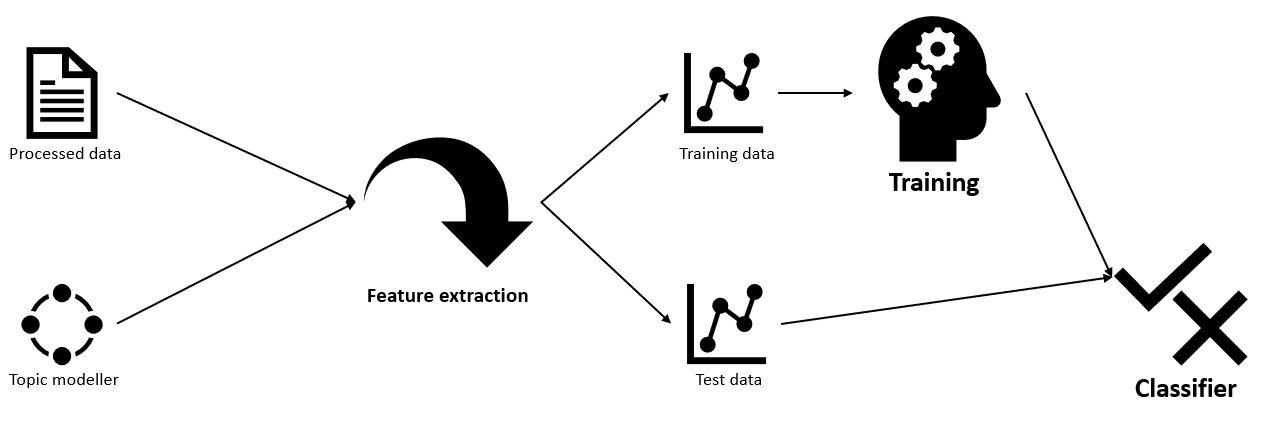
\includegraphics[width=\linewidth]{Figures/pipeline.png}
\caption{The machine learning pipeline for the classifier.}
\label{fig:cmd1}
\end{figure}

\subsection{Dataset}
The dataset used for this project is the Self-Annotated Reddit Corpus (SARC) \cite{khodakLargeSelfAnnotatedCorpus2018}. SARC provides large-scale sets of Reddit comments with markers for sarcasm representing ground truths. A comment is marked as sarcastic if the original comment included the annotation "/s". This is a conventional sarcasm marker for Reddit submissions, intended specifically to mitigate the ambiguity of sarcasm in text. For this project, I used a subset of 50,000 comments from SARC's \texttt{main-balanced} set. This set may include comments from any subreddit and has a balanced selection of sarcastic and non-sarcastic statements. SARC also offers an unbalanced set, where sarcastic statements make up $<$1\% of the data, a more realistic proportion, but I felt this would severely impact the classifier's ability to detect sarcastic statements.

The unprocessed data from SARC contains the following information about a comment:
\begin{itemize}
  \item Reddit ID
  \item Text body
  \item Author
  \item Score
  \item Date created
  \item Subreddit
\end{itemize}
SARC provides a CSV file linking comments to their parent posts by ID, as well as their self-annotated sarcasm status. By combining the information made available, I was able to create a local database of comments linked to their parent post and the subreddit they were posted to. The size of the full dataset made it impractical to index parent posts using the original file, so I further altered my local file by adding the title of each parent post and the description of the subreddit using the Reddit API through the Python Reddit API Wrapper (PRAW)\footnote{https://github.com/praw-dev/praw}.

Preprocessing on this data is intended to remove features in the text that would confuse the classifier during training. Empty comments, as well as those containing links, non-Unicode characters, and those that are replies to other comments rather than top-level comments are removed from the final dataset. Subreddits (preceded by "/r/"), username mentions (preceded by "/u/"), sarcasm markers ("/s"), hashtags, and any mention of the words "sarcasm" or "sarcastic" are removed from comment text, though the comments themselves are still included. Further processing is performed during training, where emoticons are replaced with textual descriptions (e.g. \textit{:)} is replaced with \textit{happy}). In addition, abbreviations are extended (e.g. \textit{doesn't} is replaced with \textit{does not}).

\subsection{Feature extraction}
Feature extraction is one of the key components of the training process. During training, features are extracted into a dictionary for each comment, which is appended to a list that becomes the target for the vectoriser that informs the classifier. The same feature extraction is performed when /u/IsThisSarcastic is summoned on Reddit, with the dictionary of features informing the classifier's decision function.
Features extracted during this process are:
\begin{itemize}
  \item N-grams
  \item Sentiment
  \item Parts of speech
  \item Capitalisation
  \item Topic modelling
  \item Reddit context
\end{itemize}
\subsubsection{N-grams}
Unigrams are formed by tokenising the comment's text using NLTK\footnote{https://www.nltk.org/}. Bigrams are formed using these tokens, and all n-grams are added to the feature dictionary.

\subsubsection{Sentiment analysis}
Sentiment is one of the major features extracted during this process. Two methods for scoring sentiment of a document are used in order to limit the impact of one scoring incorrectly. The first is SentiWordNet 3.0 \cite{baccianellaSENTIWORDNETEnhancedLexical2010}, a project that assigns a positive and negative sentiment score to every word in WordNet\footnote{https://wordnet.princeton.edu/}. The second is VADER \cite{huttoVADERParsimoniousRulebased2014}, a lexicon and rule-based tool designed for sentiment expression on social media, making it ideal for use with Reddit comments. VADER returns a value for positive, negative, neutral, and compound sentiment. For SentiWordNet, I record the difference between positive and negative sentiment for the input text, and for VADER I record all sentiment values. I also use TextBlob\footnote{https://textblob.readthedocs.io/en/dev/} to record the subjectivity of the text. This process is performed first over the comment as a whole, before splitting the comment in half and working on both halves, and finally again with the comment split into thirds. At the stages where the comment is split into parts, the contrast in sentiment between each part is also recorded.

\subsubsection{Parts of speech}
Using NLTK, the comment text is tagged with its parts of speech. The feature dictionary is then updated with the number of occurrences of nouns, adjectives, verbs, and adverbs.

\subsubsection{Capitalisation}
The number of words in ALL CAPS in the comment text is totalled. If there are at least 4 words in capitals, the feature dictionary is updated to note heavy capitalisation. Otherwise, it is updated to show normal capitalisation.

\subsubsection{Topic modelling}
Topic modelling for this project takes the form of an LDA model from Gensim\footnote{https://radimrehurek.com/gensim/index.html}. The topic modeller uses a symmetric distribution with 200 topics, with its corpus being formed by performing Porter stemming over the original comment data. During feature extraction, the comment is Porter stemmed and converted to a bag-of-words format, with the feature dictionary updated with the topics included in the given comment.

\subsubsection{Reddit context}
In order to model Reddit context, I give the classifier access to the same information the human respondents to my survey had; the comment's score, subreddit, and parent post. The score is directly added to the feature dictionary. The subreddit's description and parent post's title have their sentiments analysed in the same manner as the original comment, with their results added to the feature dictionary as well. Finally, the difference between the comment's sentiment and the subreddit's sentiment, as well as between the comment's sentiment and the post's sentiment, are both added to the feature dictionary. The idea behind this is that a sarcastic comment may be likely to have the opposite overall sentiment compared to their original post or subreddit. For example, a positive post about the weather being nice today may have a comment reading \textit{"This is terrible! I don't know what to do when it's like this!"}, which may return a more negative sentiment.

\subsection{Training process}
Following feature extraction, the vectoriser is generated from the list of feature dictionaries. The vectors are shuffled and split 70:30 to form a training and test set. The classifier is fitted to the training set and written to file. I conducted a series of experiments to establish the type of classifier I would use for this project, the details of which are in the next section.

\subsection{Reddit implementation}
This section also details the use of PRAW; although I had used it previously to get information about my dataset, this was its primary use in the project.

Reddit requires that any applications using their API authenticate with OAuth2\footnote{https://oauth.net/}. As such, running the program requires access to a Reddit account as well as an OAuth2 client secret. In the interest of privacy, this information is not present in this submission. References to \texttt{project1} in the code refer to my personal Reddit account which I used for early testing as well as generating the master file of comment data. References to \texttt{project2} refer to the account /u/IsThisSarcastic, which is used when the bot is active.

When the bot is run, it generates a stream of its mentions; inbox messages that users receive when others mention their username. When a mention is received, the mentioning comment is checked for one of two correct formats. The first is simply the bot's username as a reply to another comment, and the second is the username followed by a link to another comment. In the first case, the targeted comment is the parent of the mentioning comment; in the second, the targeted comment is the one linked to. The required information (text, score, subreddit description, and parent post title) is placed into a dictionary, and the comment is then scored by the classifier. The classifier returns a value between -1 and 1, where a positive score indicates that the comment is predicted as sarcastic. The bot then begins to build its reply to the user who summoned it. Table \ref{tab:cmd1} shows how the bot communicates different scores in its reply. Figure \ref{fig:cmd2} shows a usage example where the bot is tagged in an existing comment thread. Figure \ref{fig:cmd3} shows a usage example where the bot is provided a link to another comment, with that comment being shown in figure \ref{fig:cmd4}.

\begin{table}[H]
\begin{tabular}{|c|c|}
\hline
\textbf{Score (absolute value $\times$ 100)} & \textbf{Response}                      \\ \hline
score $\leq$ 10                                    & "It's too close to call!"        \\ \hline
10 $<$ score $\leq$ 25                            & "It's a very difficult decision"  \\ \hline
25 $<$ score $\leq$ 50                            & "It's quite a difficult decision" \\ \hline
50 $<$ score $\leq$ 75                            & "I'm fairly sure"                 \\ \hline
75 $<$ score $\leq$ 90                            & "I'm sure"                        \\ \hline
score $>$ 90                                       & "I'm certain"                    \\ \hline
\end{tabular}
\caption{How the bot's reply to its summoner changes according to the score generated by the classifier.}
\label{tab:cmd1}
\end{table}

\begin{figure}[H]
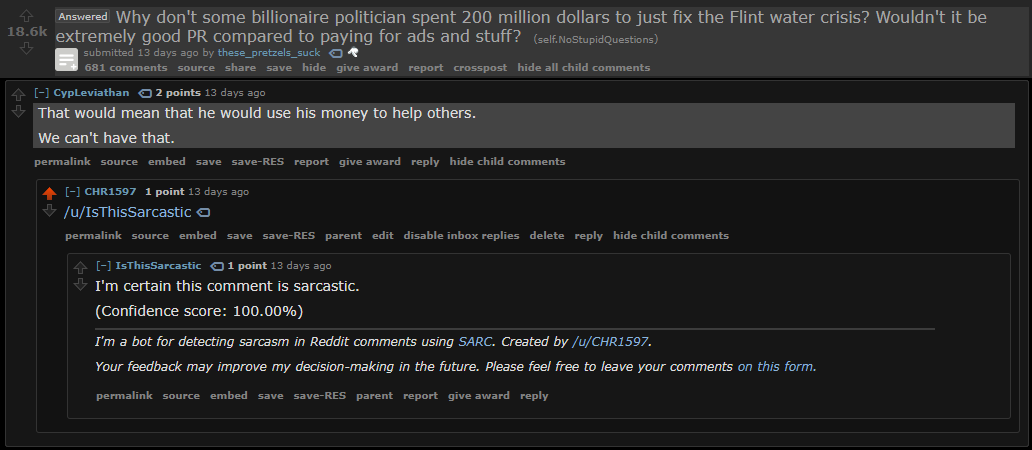
\includegraphics[width=\linewidth]{Figures/usage_example1.png}
\caption{The bot responding to a username mention in a comment thread.}
\label{fig:cmd2}
\end{figure}

\begin{figure}[H]
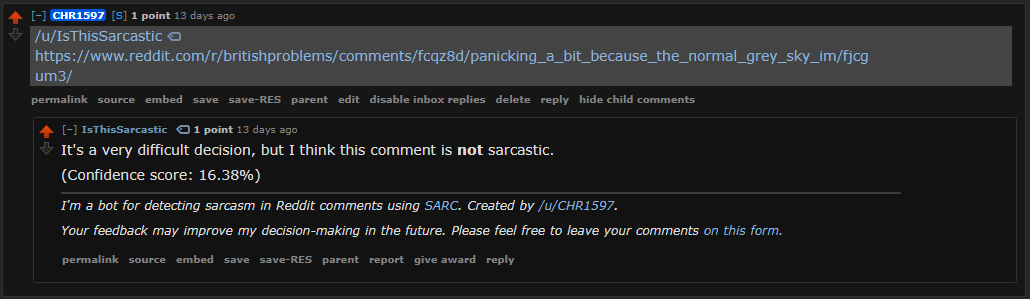
\includegraphics[width=\linewidth]{Figures/usage_example2.png}
\caption{The bot responding to a username mention with a link to another comment to judge.}
\label{fig:cmd3}
\end{figure}

\begin{figure}[H]
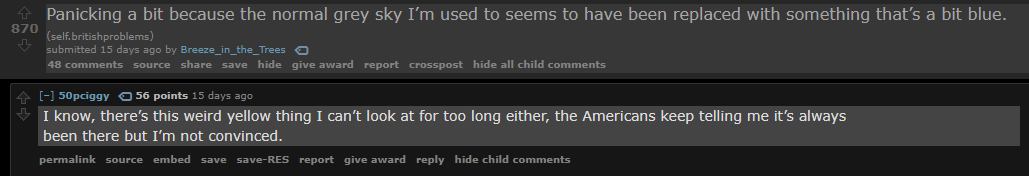
\includegraphics[width=\linewidth]{Figures/usage_example2_2.png}
\caption{The comment linked in figure \ref{fig:cmd3}.}
\label{fig:cmd4}
\end{figure}

The bot also includes a link to a feedback form in its reply. The intention here is that people who read the bot's reply may provide their opinion on whether the original comment was sarcastic. This would allow the original comment dataset to be augmented by more real-world data based on comments the bot has already judged. This takes the form of a Google Forms survey\footnote{https://forms.gle/VsvWNwCrU36YbxQp8} where respondents provide a link to the comment being judged, their personal judgement of sarcasm, and optionally what made them make that decision.

\subsection{Project Management}
While I did not formulate a specific model for time management during this project, I have had experience with agile development in industry, which led me to use those principles here. In general, my goals were set weekly, with more major goals being formed of smaller objectives. For example, the major goal for the first part of the project was to launch the survey for human respondents. Smaller goals for this included working out a useful dataset and the manner in which the questions would be asked.

Once proper development of the bot began, I divided the main goals into the same subsections as this section of the report. This gave me a clear set of objectives to meet in order to complete the implementation of the bot. As is consistent with agile practices, I performed a lot of the testing at the same time as development. I found this to be a natural way to ensure the product would always work as well as possible, as changes can be made early without requiring extensive reworking of other areas that may have required the previous implementation.

See the Discussion section for further details about the development process specifically.

\section{Results}
This section shows the results of all parts of this project. First is an analysis of the human respondents to the survey I conducted before starting development. Next is an overview of the experiments I conducted to find the optimal classifier for this problem. Finally, I examine the results I obtained from the final version of the classifier, comparing it to the earlier work I have mentioned and analysing potential error cases that prevent the classifier from scoring higher.

\subsection{Survey Responses}
As previously mentioned, I conducted a survey before starting development work to see how context affected our own ability to detect sarcasm\footnote{https://forms.gle/YAkc9tRhMVeVYJVt6}. For the full list of questions, see Appendix A. From 98 respondents, I was able to generate precision, recall, and F\textsubscript{1} scores to find the average human performance on this task. Table \ref{tab:cmd2} shows the results for human respondents with and without context.

\begin{table}[h!]
\begin{tabular}{|c|c|c|c|c|c|c|c|c|c|c|c|}
\hline
\multicolumn{6}{|c|}{\textbf{Sarcastic}}                                                                      & \multicolumn{6}{c|}{\textbf{Non-Sarcastic}}                                                                   \\ \hline
\multicolumn{3}{|c|}{\textbf{No context}}             & \multicolumn{3}{c|}{\textbf{All context}}             & \multicolumn{3}{c|}{\textbf{No context}}              & \multicolumn{3}{c|}{\textbf{All context}}             \\ \hline
\textbf{P} & \textbf{R} & \textbf{F\textsubscript{1}} & \textbf{P} & \textbf{R} & \textbf{F\textsubscript{1}} & \textbf{P} & \textbf{R} & \textbf{F\textsubscript{1}} & \textbf{P} & \textbf{R} & \textbf{F\textsubscript{1}} \\ \hline
0.83       & 0.49       & 0.61                        & 0.92       & 0.73       & 0.81                        & 0.39       & 0.77       & 0.52                        & 0.58       & 0.86       & 0.69                        \\ \hline
\end{tabular}
\caption{Details of human respondents to the sarcasm survey.}
\label{tab:cmd2}
\end{table}

From this data, we can see that the human respondents were better at detecting sarcasm when they had the context, and that they are better at detecting sarcasm than non-sarcasm. However, it is worth bearing in mind that the respondents may have been more inclined to consider a comment sarcastic than they normally would, due to having to make a decision either way.

\subsection{Classifier Experiments}
The decision of which classifier to use was a major part of the development process. Very early in development, I decided the best suite of options would come from \texttt{scikit-learn} (Pedregosa et al., 2011). This was because it provided several classification models, including the support vector and logistic regression models I saw used in my prior research.

My early tests of the library were guided by \cite{singhSarcasmDetectionStep2019}, where I attempted to use a limited corpus to train classifiers of the following types:
\begin{itemize}
  \item Linear Support Vector Classifier (Linear SVC)
  \item Gaussian Naive Bayes
  \item Logistic Regression
  \item Random Forest Classifier
\end{itemize}

The Gaussian Naive Bayes option was eliminated immediately, as its implementation in \texttt{scikit-learn} requires its input vectors to take the form of a dense matrix rather than the sparse matrix generated after feature extraction. Conversion of a sparse matrix to a dense matrix uses more memory than I had access to during development. In addition, this classifier performs the worst of the four in \cite{singhSarcasmDetectionStep2019}, and a Gaussian Naive Bayes approach is not mentioned in any of the other papers I rersearched. As such, I decided it would not be worth trying to make this approach work.

I also opted to eliminate the Random Forest approach. It performed second-worst in \cite{singhSarcasmDetectionStep2019}, and again was not featured in any of the other research I performed. That left me with a choice between Linear SVC and Logistic Regression. These two classification models both have access to a \texttt{coef\_} attribute, which provides the coefficient of features in the decision function. This allows me to view the most and least important attributes in judging a comment as sarcastic. In addition, these two models are frequently used in other works, with \cite{clicheSarcasmDetector2014} using a Linear SVC model. With my goal for this project being to out-perform that solution, it made sense to use a similar model.

The experiments I performed used two different corpora based on subsets of my final corpus. The first set of tests used 1000 comments, and the second used 10,000. The Linear SVC model had a regularisation ($C$) of 0.1 and a maximum iteration value of 10,000. The Logistic Regression model uses a limited-memory BFGS solver with a $C$ of 0.1 and 2000 maximum iterations. Both models were trained on each corpus, initially without extracting Reddit context. This gave a baseline result for how each classifier performed, before the Reddit context was introduced. Figure \ref{fig:cmd5} shows the results of this testing with 5-fold cross-validation.

\begin{figure}[h!]
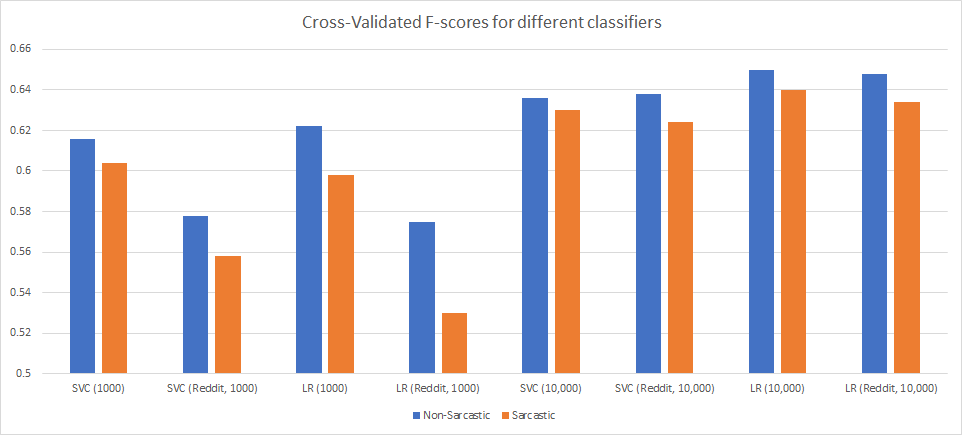
\includegraphics[width=\linewidth]{Figures/classification_report.png}
\caption{F\textsubscript{1} scores for each classifier during testing. Parenthesised is the size of the corpus and whether Reddit context was included.}
\label{fig:cmd5}
\end{figure}

Perhaps unsurprisingly, all classifiers perform significantly better with a larger training set. However, what surprised me initially was that the addition of Reddit context actually made the performance worse, with the lowest-performing classifier being the Logistic Regression machine on 1000 comments with Reddit context. This classifier returned an F\textsubscript{1} score of 0.53 for the sarcastic category and 0.575 for non-sarcastic.

With a larger corpus of 10,000 comments, the situation is quite different. The classifier versions that use Reddit context performed almost identically to those that do not. On average, a classifier with 10,000 comments is equally adept at detecting non-sarcastic comments with or without context, and is worse at detecting sarcasm by a margin of 0.006 F\textsubscript{1} score. This negligible difference convinced me that a larger corpus made context more useful. In addition, a 10,000-comment corpus makes the Logistic Regression model outperform the Linear SVC model. At this point, the Linear SVC model often failed to fully converge despite having 5 times the maximum iterations of the Logistic Regression model. This would suggest that the Linear SVC model was unable to find the "most similar" comments in opposing classes in 10,000 attempts. The Logistic Regression model draws its decision boundary by taking every data point into account, so it did not have this problem. This may explain why the Logistic Regression model scored higher at this stage of testing, but I felt that the problem would only be exacerbated at the full scope of the corpus of 50,000 comments.

As mentioned previously, the classifier models I used for these experiments have a \texttt{\_coef} attribute, representing the coefficient of features in the decision function. After each individual classifier was generated, I had details of its coefficients printed to establish what factors are most important for classifying a comment as sarcastic. What these experiments demonstrated was that by far the most important factor was the N-grams. In other words, sarcasm appears to be best-demonstrated by vocabulary.

This process also brought up a potential problem with the data I used. On one occasion, a sample classifier reported a topic in its topic modeller made up of Dutch words, as seen in figure \ref{fig:dutch}. This shows that some of the comments from SARC are non-English, potentially adding some unnecessary noise for the vast majority of cases that are in English. \cite{clicheSarcasmDetector2014} recognised this problem, solving it by only using tweets whose location data came from cities in the USA. I opted to try and solve the problem using TextBlob's \texttt{detect\_language()} function, but found to my surprise that it returned an HTTP 429 error. This function in TextBlob goes to Google's API, which has its own rate limit. Adhering to that limit would make preprocessing of data take too long to be feasible, so I then tried an offline approach using the \texttt{langdetect} library\footnote{https://pypi.org/project/langdetect/}. This returned results quickly, but was too inaccurate to be useful. Figure \ref{fig:lang} shows two English phrases marked as French and Somali respectively. I therefore decided that this problem would have such a limited effect on the final results, if any at all, that it would not be a serious issue if left unsolved.

\begin{figure}[h!]
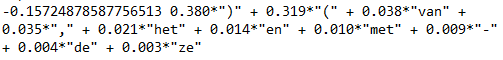
\includegraphics[width=\linewidth]{Figures/topic_example.png}
\caption{A topic modelled by one of the experimental classifiers, showing a vocabulary of Dutch words.}
\label{fig:dutch}
\end{figure}

\begin{figure}[h!]
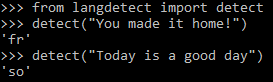
\includegraphics[width=\linewidth]{Figures/language_inaccurate.png}
\caption{\texttt{langdetect} showing two example English phrases as French and Somali respectively.}
\label{fig:lang}
\end{figure}

\subsection{Final Results}
The final classifier uses a Logistic Regression model with a limited-memory BFGS solver, a $C$ of 0.1, and 2000 maximum iterations. Table \ref{tab:cmd3} presents the performance results of /u/IsThisSarcastic alongside human results, similar sarcasm detection approaches, and state-of-the-art deep learning approaches.

\begin{table}[h!]
\begin{tabular}{|c|c|c|c|l|}
\hline
\textbf{Classifier}                    & \textbf{Precision} & \textbf{Recall} & \textbf{F\textsubscript{1}} & \textbf{Accuracy} \\ \hline
\textbf{Human}                         & 0.92               & 0.73            & 0.81                        & -                 \\ \hline
\textbf{\cite{gonzalez-ibanezIdentifyingSarcasmTwitter2011}} & -                  & -               & -                           & 0.65              \\ \hline
\textbf{\cite{clicheSarcasmDetector2014}}                 & -                  & -               & 0.60                        & -                 \\ \hline
\textbf{\cite{tayReasoningSarcasmReading2018}}             & 0.697              & 0.694           & 0.695                       & 0.699             \\ \hline
\textbf{\cite{hazarikaCASCADEContextualSarcasm2018}}        & -                  & -               & 0.77                        & 0.77              \\ \hline
\textbf{/u/IsThisSarcastic}            & \textbf{0.64}               & \textbf{0.68}            & \textbf{0.66}                        & \textbf{0.66}              \\ \hline
\end{tabular}
\caption{Comparison of the performance between /u/IsThisSarcastic, human respondents to the survey, and various examples of previous work.}
\label{tab:cmd3}
\end{table}

While I do not have full results for all of the previous solutions, what we can see from these results is that /u/IsThisSarcastic out-performs \cite{clicheSarcasmDetector2014} in F\textsubscript{1} score by 6 percentage points. It also has better accuracy than the seminal work from \cite{gonzalez-ibanezIdentifyingSarcasmTwitter2011}. In addition, /u/IsThisSarcastic scores within 4 percentage points of the state-of-the-art deep learning solution proposed by \cite{tayReasoningSarcasmReading2018}. Perhaps unsurprisingly, the human respondents to my survey perform better than any automated solutions.

\section{Discussion}
This section serves as my personal response to the development and results of this project.

\subsection{Analysis of Results}
With the reported results of /u/IsThisSarcastic, I have met my goal of out-performing the supervised learning-based sarcasm detector designed by \cite{clicheSarcasmDetector2014}. However, it is worth noting that during the classifier experiment phase, by the time I was testing with 10,000 comments I was already out-performing the F\textsubscript{1} score of 0.60 achieved by \cite{clicheSarcasmDetector2014}. This would suggest that the performance gains of /u/IsThisSarcastic are not necessarily related to my inclusion of contextual information, but may instead be related to the corpus used or improvements to the \texttt{scikit-learn} libraries.

However, the best-performing state-of-the-art solutions are those that model context. Indeed, the solution by \cite{tayReasoningSarcasmReading2018}, the performance of which /u/IsThisSarcastic is less than 4 percentage points away from, is one of the few sarcasm detectors for social media posts that does not attempt to model context. In this way, we can broadly divide "sarcasm detectors" into categories of supervised learning and deep learning. In both of these categories, the solutions that model context perform better than those that do not.

One difference between the style of context modelling I chose and that used by solutions like CASCADE \cite{hazarikaCASCADEContextualSarcasm2018} is that I opted to emulate the "context" a human reader would be likely to establish when reading a Reddit comment. This led me to focus on a comment's score, the post being commented on, and the subreddit the post is on. State-of-the-art solutions such as CASCADE and \cite{poriaDeeperLookSarcastic2017} instead opt to model context using personality analysis of comment authors. This approach better emulates the way we use sarcasm in person, where we learn what someone might be likely to say in earnest over time to establish what their "version" of sarcasm sounds like. However, I decided that this style of context modelling was not only well-explored already, but was also somewhat unrealistic for comparison to human performance. The average Reddit user will probably not view the profile of a comment author to establish their personality if there are more immediately available context clues to inform whether the comment was sarcastic. In addition, performing contextual analysis in this way is very time-consuming when dealing with Reddit, as their API has a strict rate limit of 30 requests per minute. CASCADE's implementation involves retrieving every comment made by a user to form their personality map. With some users making thousands of comments, this process could take several hours purely through API rate limits. This would also limit /u/IsThisSarcastic's usability as a summonable Reddit bot, as every comment written by the user in question would need to be analysed, rather than the current implementation which requires significantly less information from Reddit.

User feedback is another factor in the results from /u/IsThisSarcastic. Readers can use the survey linked in each of the bot's comments to leave feedback on its decisions. This is intended to use the as-yet unbeaten human capability for detecting sarcasm to add new comments to a potential future dataset, thereby improving the bot's accuracy. The survey is naturally ever-evolving, but at time of writing, the survey would indicate that, in practice, the bot is only accurate 25\% of the time. This represents a large discrepancy with the reported performance over the full corpus. I believe this is down to two factors: firstly, most users will not bother leaving feedback, especially if the bot's comment is just part of a conversation they were already reading; secondly, when a user is compelled to leave feedback, it is probably because they disagree with the bot's judgement. These problems may be because there is no individual benefit to a user for leaving feedback, so the natural response bias that causes extreme opinions to be more prevalent in survey respondents means that there are relatively few total responses, and those that do exist are mostly negative.

\subsection{Reflection on Development}
This is not to say that /u/IsThisSarcastic is without limitations, of course. A more specialised, custom deep learning approach would appear to give better final results, but I opted to go with \texttt{scikit-learn} implementations instead. This is because I was already entering new personal territory with machine learning, and felt that the time required to learn enough theory to propose a novel approach would impact my ability to develop a working system.

I would say my lack of experience in the area of machine learning is the main limitation of this project. I spent a lot of time in the early development stages making assumptions about how supervised classifiers work, mainly in that my initial plan was to alter the \texttt{scikit-learn} classifier implementations to have them accept context for me. I realised this idea would not work before attempting it, but it was still what I expected to do as late as December.

As a result, much of the real development for this project took place after Christmas, with very little work from before then actually featuring in the final code. I feel that if I had been more aware earlier on of what this project would require, I could have had more time to develop the specifics of the machine learning side.

While the Reddit implementation went more smoothly, there are still some limitations imposed by working with a third-party API. During development, the major hurdle was the aforementioned rate limiting. The additions I needed to make to the SARC dataset required multiple connections to Reddit for each comment in the corpus. PRAW approximates adherence to the rate limit by limiting requests to one every two seconds, so for the corpus of 50,000 comments I used where each required five requests to Reddit, I had to spend almost six full days appending to the dataset.

The requirements of working with the Reddit API also impacted the running of the bot itself, which is another area I would like to improve. Currently, /u/IsThisSarcastic is registered with Reddit as a script app. This means that it should run on only one system for personal administration. As a result, I have to run the process on my machine to have the bot reply to any comments. Ideally, I would like the bot to run on a web server for constant accessibility. This would also allow a custom method for linking feedback to a specific comment, rather than the current implementation of a Google Forms survey. However, this implementation would have required me to register with Reddit as a web app, which would have needed me to develop the site first as Reddit requires web apps to register with an existing domain. I felt that my priority was getting a working bot first, so this was not possible in time.

With these limitations and improvements in mind, I am generally satisfied with the development and results of this project. I believe I have developed a system that pairs well with its intended use as a Reddit bot to perform multifaceted but lightweight sarcasm detection on arbitrary documents with an encouraging level of success.

\section{Conclusion}
This project introduced /u/IsThisSarcastic, an autonomous Reddit bot that can be summoned to deduce whether any given comment is sarcastic or not. It extracts lexical, syntactic, and semantic information from the comment's text, and contextual information from the Reddit environment. Using a Logistic Regression classifier trained on a corpus of Reddit comments, /u/IsThisSarcastic out-performs similar supervised learning-based sarcasm detectors, and approaches the performance of some state-of-the-art deep learning solutions. This shows that the contextual information that improves human ability to discern sarcasm can also impact the abilities of automated sarcasm detectors.
\clearpage

\begin{footnotesize}
\bibliography{references}
\bibliographystyle{apalike}
\end{footnotesize}

\newpage
\pagenumbering{arabic}
\renewcommand*{\thepage}{A\arabic{page}}
\appendix

\section{Instructions for Running}
/u/IsThisSarcastic was developed using Python 3.8.1, and requires the following optional packages (run \texttt{pip install <name>}):
\begin{itemize}
	\item \texttt{gensim}
	\item \texttt{nltk}
	\item \texttt{numpy}
	\item \texttt{praw}
	\item \texttt{textblob}
	\item \texttt{vaderSentiment}
\end{itemize}

Generating new classifiers also requires the libraries \texttt{scipy} and \texttt{sklearn}.

A file titled \texttt{praw.ini} is required for the PRAW library to log into Reddit as a specific user. As mentioned in section 3.5, the Reddit API requires any application that uses it to register with Reddit using OAuth2. As such, running this program requires a Reddit account to which any comments will be posted. When the application has been registered with Reddit, you will be given a client ID and client secret. Once you have this information, the \texttt{praw.ini} file should be made to this specification:

\begin{verbatim}
[project2]
client_id = <Client ID>
client_secret = <Client Secret>
user_agent = <User agent string>
username = <Account username>
password = <Account password>
\end{verbatim}

With \texttt{praw.ini} in the \texttt{code/final} directory, run
\texttt{detector.py}
from the same directory. When the console reads \texttt{Ready.}, replying to a Reddit comment with the username of the connected account will prompt the bot to reply. Adding a link to another Reddit comment will prompt it to analyse the linked comment instead.

To generate a new classifier, run:
 
\texttt{train.py <include\_reddit> <classifier\_type>}

where \texttt{<include\_reddit>} is 0 or 1 to indicate whether Reddit context should be included, and \texttt{<classifier\_type>} is 1 or 2, indicating a Linear SVC or Logistic Regression model respectively.

\section{Survey questions}
\begin{enumerate}
	\item "Wow I wonder who could be behind this?"
	\begin{itemize}
		\item Subreddit: worldnews
		\item Description: "/r/worldnews is for major news from around the world except US-internal news / US politics"
		\item Score: 37
		\item Post: "North Korea's internet is offline; massive DDOS attack presumed"
	\end{itemize}

	\item "This is incredible, everyday we're seeing more people on the Bitcoin train."
	\begin{itemize}
		\item Subreddit: Bitcoin
		\item Description: "Bitcoin is the currency of the Internet: a distributed, worldwide, decentralized digital money."
		\item Score: 15
		\item Post: "Jack Dorsey says Square will accept bitcoin"
	\end{itemize}

	\item "Best actress, ever."
	\begin{itemize}
		\item Subreddit: Celebs
		\item Description: "For beautiful female celebrities."
		\item Score: -8
		\item Post: "Zooey Deschanel"
	\end{itemize}

	\item "I'm certain this will be of particular use to people studying mechanical engineering."
	\begin{itemize}
		\item Subreddit: canada
		\item Description: "Canada - the country, people, culture, and yeah, the hockey, snow and all things Canadian."
		\item Score: 3
		\item Post: "University of Winnipeg makes indigenous course a requirement"
	\end{itemize}

	\item "what a rough life"
	\begin{itemize}
		\item Subreddit: EDM
		\item Description: "The front page of the internet's home for all things EDM."  [EDM = Electronic Dance Music]
		\item Score: -17
		\item Post: "Drugs, sleeplessness, isolation: the downside of being a dance musician"
	\end{itemize}

	\item "If they can do it in India, they can do it in America."
	\begin{itemize}
		\item Subreddit: conspiracy
		\item Description: "We hope to challenge issues which have captured the public’s imagination, from JFK and UFOs to 9/11."
		\item Score: 10
		\item Post: "India just turned off mobile internet for 63 million citizens amid protests in Ahmedabad"
	\end{itemize}

	\item "It's clearly a Rolls Royce... Just look at the grill."
	\begin{itemize}
		\item Subreddit: Shitty\_Car\_Mods
		\item Description: "Post pictures of cars with terrible mods"
		\item Score: 8
		\item Post: "Poor Charger."
	\end{itemize}

	\item "The sun is gonna destroy us in a few billion years anyways, so why does it matter if we die out in the next few centuries?"
	\begin{itemize}
		\item Subreddit: politics
		\item Description: "/r/Politics is for news and discussion about U.S. politics."
		\item Score: 5
		\item Post: "Gary Johnson Wants to Ignore Climate Change Because the Sun Will Destroy the Earth One Day"
	\end{itemize}

	\item "Wow I think that is the most interesting things ive ever read on this sub"
	\begin{itemize}
		\item Subreddit: todayilearned
		\item Description: "You learn something new every day; what did you learn today?"
		\item Score: 1
		\item Post: "TIL Namco has a US patent on having mini-games inside of their game's loading screens; this is why most games have such boring loading screens"
	\end{itemize}

	\item "Misery loves company."
	\begin{itemize}
		\item Subreddit: AskReddit
		\item Description: "r/AskReddit is the place to ask and answer thought-provoking questions."
		\item Score: 7
		\item Post: "Why do some people think not having kids is "selfish"?"
	\end{itemize}
\end{enumerate}

\end{document}